% Nejprve uvedeme tridu dokumentu s volbami
\documentclass[czech,master]{diploma}
% Dalsi doplnujici baliky maker
\usepackage[autostyle=true,czech=quotes]{csquotes} % korektni sazba uvozovek, podpora pro balik biblatex
\usepackage[backend=biber, style=iso-numeric, alldates=iso]{biblatex} % bibliografie
\usepackage{dcolumn} % sloupce tabulky s ciselnymi hodnotami
\usepackage{subfig} % makra pro "podobrazky" a "podtabulky"
\usepackage[cpp]{diplomalst}
\usepackage{amsmath}
\usepackage{amsmath}
\usepackage{amssymb}
\usepackage{bussproofs}

% Zadame pozadovane vstupy pro generovani titulnich stran.
\ThesisAuthor{Bc. Jakub Koběrský}

\ThesisSupervisor{Ing. Martin Kot, Ph.D.}

\CzechThesisTitle{Komponenta výukového serveru MAV - Kalkulus komunikujících systémů}

\EnglishThesisTitle{Component of Learning Server for Modeling and Verification - Calculus of Communicating Systems}

\SubmissionYear{2026}

\ThesisAssignmentFileName{TheSisSpecification.pdf}

% Pokud nechceme nikomu dekovat makro zapoznamkujeme.
\Acknowledgement{TODO}

\CzechAbstract{TODO}

\CzechKeywords{diplomová práce; TODO}

\EnglishAbstract{TODO}

\EnglishKeywords{master thesis; TODO}

\AddAcronym{CCS}{Calculus of Communicating Systems, kalkulus komunikujících systémů}
\AddAcronym{SOS}{Structural Operational Semantics, strukturální operační sémantika}
\AddAcronym{LTS}{Labelled Transition System, ohodnocený přechodový systém}
\AddAcronym{AST}{Abstract Syntax Tree, abstraktní syntaktický strom}
\AddAcronym{HML}{Hennessy-Milner Logic}
\AddAcronym{LTL}{Linear Temporal Logic}
\AddAcronym{CTL}{Computation Tree Logic}
\AddAcronym{CSP}{Communicating Sequential Processes}
\AddAcronym{ACP}{Algebra of Communicating Processes}
\AddAcronym{MaV}{Modelování a verifikace}
\AddAcronym{CAAL}{Algebra of Communicating Processes}
\AddAcronym{CWB}{Edinburgh Concurrency Workbench}
\AddAcronym{UX}{User experience, Uživatelská přívětivost}
\AddAcronym{UI/UX}{User interface / User experience, Uživatelské rozhraní / Uživatelská přívětivost}
\AddAcronym{PWA}{Progressive web app, Progresivní webová aplikace}
\AddAcronym{SPA}{Single Page Application}
\AddAcronym{JS}{JavaScript}
\AddAcronym{TS}{TypeScript}
\AddAcronym{CSS}{Cascading Style Sheets, kaskádové styly}
\AddAcronym{HTML}{HyperText Markup Language}
\AddAcronym{JSON}{JavaScript Object Notation}
\AddAcronym{HMR}{Hot Module Replacement}

\addbibresource{citations.bib}

% Novy druh tabulkoveho sloupce, ve kterem jsou cisla zarovnana podle desetinne carky
\newcolumntype{d}[1]{D{,}{,}{#1}}


% Zacatek dokumentu
\begin{document}

% Nechame vysazet titulni strany.
\MakeTitlePages

% Jsou v praci obrazky? Pokud ano vysazime jejich seznam a odstrankujeme.
% Pokud ne smazeme nasledujici dve makra.
\listoffigures
\clearpage

% Jsou v praci tabulky? Pokud ano vysazime jejich seznam a odstrankujeme.
% Pokud ne smazeme nasledujici dve makra.
\listoftables
\clearpage

% A nasleduje text zaverecne prace.
\chapter{Úvod}
\label{sec:Introduction}
S neustálým rozvojem informačních technologií pronikají počítačové systémy do všech aspektů lidského života, kde se stále častěji setkáváme s reaktivními systémy.
Příkladem těchto systémů mohou být běžné webové služby, nápojové automaty, ale i kritické řídicí systémy v dopravě, zdravotnictví a průmyslu. 
Tyto systémy nejsou navrženy k jednorázovému výpočtu a následnému ukončení, ale k~neustálé interakci se svým okolím. 
Vzhledem k jejich paralelní a nedeterministické povaze je~zaručení jejich bezchybného chování pomocí tradičních způsobů testování prakticky nemožné. 

Pro zaručení korektnosti systémů se proto využívají matematicky podložené metody formální verifikace. 
Jednou ze základních metod v této oblasti je kalkulus komunikujících systémů, který představil britský informatik Robin Milner. 
Tento formální jazyk umožňuje modelovat složité konkurentní systémy pomocí propojení jednoduchých nezávislých procesů, zkoumat jejich chování přes strukturální operační sémantiku a vizualizovat je pomocí ohodnocených přechodových systémů.

Výuka těchto systémů ale často naráží na překážky, a to zejména v prvotních hodinách, kdy se~studenti setkají s formálními matematickými důkazy. 
Existující nástroje jsou totiž často navrženy pro potřeby pokročilé analýzy, nejsou tedy přizpůsobeny pro interaktivitu a výuku úplných základů.
Cílem této diplomové práce je proto navrhnout a implementovat výukovou webovou aplikaci, která studentům usnadní pochopení základních problémů z oblasti formální verifikace systémů. 
Práce si klade za cíl vytvořit dynamickou a uživatelsky přívětivou aplikaci, ve které mohou uživatelé experimentovat s vlastními modely a vizualizovat jejich chování. 
Aplikace zajišťuje kontrolu syntaxe zadaných CCS výrazů, zobrazení jejich syntaktických stromů a poskytuje uživateli prostředí pro~interaktivní a kontrolovanou tvorbu formálních důkazů podle pravidel SOS. 
Vedle toho systém umožňuje automatické generování odpovídajících LTS grafů a simulaci běhu jednotlivých procesů. 
Aby byla aplikace co nejpřístupnější, obsahuje také sadu připravených ukázkových vstupů.

Text práce je rozdělen do pěti na sebe navazujících kapitol. 
V kapitole \ref{sec:reaktivni_systemy} se probírá teoretický základ reaktivních systémů a detailně popisuje formalismus kalkulu komunikujících systémů, ohodnocených přechodových systémů a strukturální operační sémantiky. 
Kapitola \ref{sec:analyza_pozadavku} analyzuje existující řešení a definuje funkční i nefunkční požadavky na vyvíjenou aplikaci. 
V kapitole \ref{sec:technologie} jsou představeny použité moderní webové technologie a knihovny, jako jsou React.js, Peggy.js a Cytoscape.js. 
Kapitola \ref{sec:navrh} se věnuje celkovému architektonickému návrhu řešení a uživatelského rozhraní.
V neposlední řadě popisuje kapitola \ref{sec:implementace} samotnou implementaci výpočetní logiky, datových struktur, algoritmů a~způsob nasazení aplikace.

Výsledná verze aplikace je za pomoci nástroje Github Pages \cite{github_pages_2026_github} nazasena na veřejné adrese \\ \texttt{https://ccs.koberskyj.cz/}.

Během vývoje této práce byla využívána umělá inteligence, konkrétně model Gemini pro jazykovou korekturu textu a pro asistenci při programování, zejména tedy při ladění aplikace v prostředí React.js.

\endinput

\chapter{Kalkulus komunikujících systémů}

\endinput
\chapter{Analýza požadavků}
\label{chap:analyza_pozadavku}

Tato kapitola se věnuje analýze požadavků na vyvíjenou webovou aplikaci, jejímž cílem je podpora výuky vybraných problémů z oblasti formální verifikace systémů. 
V následujících sekcích je specifikován primární účel aplikace, zhodnocení existujících nástrojů a podrobná specifikace funkčních i nefunkčních požadavků definovaných na základě zadání.

\section{Účel aplikace}
\label{sec:ucel_aplikace}
Primárním účelem vyvíjené aplikace je sloužit jako interaktivní vizuální pomůcka pro studenty předmětu Modelování a verifikace (MaV), případně obdobných kurzů zaměřených na formální metody. 
Teorie formální verifikace a modelování konkurentních systémů pomocí kalkulu komunikujících systémů (CCS) může být pro studenty zpočátku složitější na pochopení, zejména pokud nemají k dispozici adekvátní nástroj pro vizualizaci chování těchto systémů. 

Hlavním přínosem aplikace je provedení studenta prvními fázemi studia problematiky. 
Uživatel si může interaktivně vyzkoušet sestrojení ohodnoceného přechodového systému (LTS) na základě definovaných CCS výrazů, případně krok za krokem dokazovat platnost přechodů za užití pravidel strukturální operační sémantiky (SOS).

Jedním z hlavních cílů aplikace je tento vzdělávací proces usnadnit poskytnutím okamžité vizuální zpětné vazby. 
Aplikace umožní studentům experimentovat s vlastními procesy, vizualizovat jejich syntaktickou strukturu, krokovat jejich běh a především interaktivně budovat formální důkazy pomocí SOS pravidel. 
Díky tomu si mohou uživatelé lépe představit abstraktní principy synchronizace, nedeterminismu a komunikace mezi procesy.

\section{Analýza existujících řešení}
\label{sec:analyza_existujicich_reseni}
Oblast formální verifikace a analýzy systémů popsaných pomocí CCS již disponuje řadou aplikací. 
Většina z nich však byla navržena primárně pro výzkumné nebo průmyslové účely, nikoliv explicitně jako pomůcky pro začátečníky. 
Mezi nejvýznamější programy v kontextu existujícího softwaru je vhodné zmínit následující aplikace.

\subsection{Concurrency Workbench Aalborg (CAAL)}
Jako nejvýznamnější moderní nástroj lze uvést CAAL (Concurrency Workbench Aalborg) \cite{caal}. 
Jedná se o komplexní webovou aplikaci umožňující specifikaci procesů v CCS, generování LTS, ověřování bisimulačních ekvivalencí a model checking pomocí modální logiky.
Je to poměrně intuitivní nástroj, který se i během výuky předměnu používá, obsahuje však i určité limity. 
Hlavní nevýhodou je absence podpory pro dokazování přechodů pomocí jednotlivých SOS pravidel, což omezuje jeho využití v úvodních fázích výuky.
Při generování LTS grafů navíc CAAL využívá algoritmy optimalizované spíše pro rozsáhlé stavové prostory, což má za následek horší přehlednost u menších výukových příkladů. 
Nástroj rovněž neposkytuje vizualizaci abstraktního syntaktického stromu (AST), která je pro pochopení sémantiky a priorit operátorů klíčová.

\subsection{Edinburgh Concurrency Workbench (CWB)}
Historicky důležitým nástrojem, který definoval standard pro automatizovanou analýzu CCS, je CWB \cite{CWB}. 
Ačkoliv se jedná o spolehlivý software s vysokým výkonem, v dnešní době již není dále vyvíjen.
Jeho zásadním nedostatkem pro účely moderní výuky je zastaralé uživatelské rozhraní založené výhradně na příkazové řádce. 
Neposkytuje žádnou formu interaktivní vizualizace grafů či syntaktických stromů, což jej činí pro podporu výuky těžko přístupným.

\subsection{Zhodnocení a přínos nové aplikace}
Z analýzy existujících řešení vyplývá, že hlavním nedostatkem je přílišná komplexita uživatelského rozhraní a absence nástrojů zaměřených čistě na pochopení základních principů (např. krokové budování SOS důkazů a vizualizace AST).
Hlavním přínosem nového řešení je tak primárně zaměření na výuku. 
Aplikace nabídne validaci syntaxe v reálném čase, možnost vizuální nápovědy při volbě SOS pravidel a moderní, čisté prostředí. 
Stává se tak vhodným doplňkem (zejména pro úvodní přednášky a cvičení) k robustnějším nástrojům, nikoliv však jejich náhradou.

\section{Funkční požadavky}
\label{sec:funkcni_pozadavky}

Funkční požadavky přímo definují chování a možnosti vyvíjené aplikace. Vycházejí z oficiálního zadání diplomové práce a jsou rozšířeny o potřeby nezbytné pro reálné nasazení ve výuce:

\begin{enumerate}
    \item \textbf{Zadávání a syntaktická analýza CCS výrazů}
    \begin{itemize}
        \item Systém musí obsahovat textový editor pro zápis zdrojového kódu (procesních definic) v syntaxi jazyka CCS.
        \item Aplikace musí v reálném čase provádět syntaktickou analýzu vstupu a vizuálně upozorňovat uživatele na případné chyby (např. chybějící závorky, nepovolené znaky, nedefinované procesy).
        \item K zadanému a syntakticky korektnímu výrazu musí systém umožnit vygenerování a zobrazení syntaktického stromu (AST), reprezentujícího hierarchickou strukturu výrazu a prioritu operátorů.
    \end{itemize}
    
    \item \textbf{Interaktivní konstrukce odvozovacího stromu (SOS)}
    \begin{itemize}
        \item Pro uživatelem zvolené procesy $X$ a $Y$ a akci $\alpha$ musí systém umožnit uživateli sestavit formální důkaz přechodu $X \xrightarrow{\alpha} Y$ na základě axiomů a odvozovacích pravidel strukturální operační sémantiky.
        \item Tento proces musí probíhat interaktivně: uživatel postupně vybírá pravidla aplikovatelná na daný podvýraz, včetně jejich příslušných parametrů.
        \item Aplikace musí nabízet dva režimy podpory výuky:
        \begin{enumerate}
            \item \textit{Režim bez nápovědy:} Uživatel provádí volbu pravidel samostatně. V případě chybného kroku jej aplikace pouze upozorní,  že dané pravidlo s příslušnými parametry nelze použít.
            \item \textit{Režim s nápovědou:} Systém na základě aktuálního stavu výrazu interaktivně filtruje a zvýrazňuje pouze ta SOS pravidla, která jsou syntakticky aplikovatelná, a omezuje výběr parametrů na validní možnosti.
        \end{enumerate}
    \end{itemize}
    
    \item \textbf{Generování a vizualizace ohodnoceného přechodového systému (LTS)}
    \begin{itemize}
        \item Na základě zadaného CCS výrazu musí systém vygenerovat odpovídající stavový prostor a zobrazit jej jako orientovaný graf, kde vrcholy reprezentují stavy prostoru a orientované hrany jednotlivé akce.
        \item Systém musí být odolný vůči zacyklení v případech, kdy je generovaný LTS nekonečný (např. vlivem neomezeného vytváření nových paralelních komponent nebo nezastavené rekurze). Generování musí být omezeno či přizpůsobeno tak, aby nedošlo k zamrznutí uživatelského rozhraní.
    \end{itemize}
    
    \item \textbf{Simulace běhu procesů}
    \begin{itemize}
        \item Aplikace musí obsahovat interaktivní simulátor umožňující manuální krokování běhu procesu napříč vygenerovaným LTS grafem.
        \item Uživatel musí mít možnost v každém stavu zvolit, kterou z dostupných akcí chce provést.
        \item Simulátor musí umožňovat návrat o krok zpět, případně celou simulaci vrátit do výchozího stavu.
        \item Při analýze paralelních procesů (využívajících operátor $|$) simulátor vizuálně demonstruje nezávislé provádění akcí i interní komunikaci (handshake) přes komplementární porty (např. $\alpha$ a $\overline{\alpha}$), vedoucí ke vzniku tiché akce $\tau$.
    \end{itemize}
    
    \item \textbf{Předdefinované ukázkové vstupy}
    \begin{itemize}
        \item Systém musí obsahovat sadu předpřipravených příkladů demonstrujících použití jednotlivých operátorů CCS a typických situací ve formální verifikaci.
        \item Tyto ukázky musí být možné načíst na jedno kliknutí bez nutnosti psaní kódu, což urychlí seznámení uživatele s aplikací.
    \end{itemize}
\end{enumerate}

\section{Vedlejší požadavky}
\label{sec:vedlejsi_pozadavky}

Vedlejší (nefunkční) požadavky definují vlastnosti systému, které nesouvisejí přímo s hlavní funkcionalitou verifikace, ale jsou klíčové pro celkovou uživatelskou přívětivost (UX), stabilitu a moderní standardy vývoje webových aplikací.

\begin{enumerate}
    \item \textbf{Podpora offline režimu a PWA architektura:} 
    Aplikace by měla být navržena jako progresivní webová aplikace (PWA). 
    Logika výpočtů a zpracování CCS by mělo probíhat primárně na straně klienta, což umožní plnohodnotné využití nástroje i bez stabilního připojení k internetu. 
    Ukládání rozpracovaných příkladů by mělo být řešeno pomocí lokálního úložiště prohlížeče, aby bylo možné uchovat rozpracovaný stav přímo v prohlížeči i bez přístupu k internetu.
    
    \item \textbf{Lokalizace uživatelského rozhraní (i18n):} 
    Aplikace by měla podporovat minimálně češtinu a angličtinu. 
    Přepnutí jazyka musí proběhnout plynule bez nutnosti opětovného načtení celé stránky. 
    Architektura aplikace by měla umožňovat snadné přidání dalších jazyků v budoucnosti.
    
    \item \textbf{Export a vizualizace dat:} 
    Aplikace musí umožnit export vygenerovaných syntaktických stromů a LTS grafů. 
    Ideální je i podpora exportu do rastrových (PNG) i vektorových (SVG) formátů, aby je studenti mohli snadno začlenit do svých úkolů či prací. 
    Vhodný je i export struktury do strojově čitelného formátu (např. JSON).
    
    \item \textbf{Sdílení programů:} 
    Systém musí poskytovat mechanismus pro snadné sdílení vytvořených procesů. 
    Uživatel by měl mít možnost jednoduše zkopírovat kód nebo sdílet rozpracované řešení, což zefektivní komunikaci mezi uživateli.
    
    \item \textbf{Přístupnost a responsivní design:} 
    Přestože se předpokládá primární využití na desktopových zařízeních, rozhraní musí být responsivní a funkční i na mobilních telefonech a tabletech. 
    Aplikace by měla být také přístupná podle zákonu o přístupnosti, platném od roku 2025. I přesto, že se na tuto aplikaci zákon momentálně nevztahuje, měla by respkeptovat metodiku WCAG 2.2. \cite{pristupnostWebu}
    
    \item \textbf{Integrovaná nápověda a dokumentace:} 
    Součástí uživatelského rozhraní musí být kontextová nápověda (např. tooltipy vysvětlující jednotlivá SOS pravidla) a centrální dokumentace, která stručně objasní jak ovládání samotné aplikace, tak základní pojmy.
    
    \item \textbf{Moderní UI/UX s využitím animací:} 
    Vizuální stránka by měla působit čistě a moderně. 
    Přechody stavů a úpravy grafů by měly být podpořeny plynulými animacemi. 
    Tyto animace nemají plnit pouze estetickou funkci, ale také sloužit ke snížení kognitivní zátěže uživatele (např. plynulé zobrazení kroků při animaci průchodu grafem).

    \item \textbf{Možnost uzamknutí programu:}
    Rozhraní by mělo umožnit uzamčení textového editoru, zadání SOS důkazů a dalších prvků aplikace. 
    Toto uzamčení bude sloužit zejména jen jako ochrana proti nechtěným změnám, uživatel si ji může libovolně u programů aktivovat či deaktivovat.

    \item \textbf{Strukturální redukce LTS grafu:}
    Systém by měl uživateli nabídnout možnost zjednodušit generované grafy a stromy, například automatickým odstraňováním zbytečných \texttt{Nil} procesů či aplikací základních pravidel strukturální kongruence.

\end{enumerate}

\endinput
\chapter{Použité technologie}
\label{sec:technologie}

V této kapitole jsou popsány softwarové nástroje, knihovny a technologie, které byly využity při návrhu a implementaci praktické části této diplomové práce. 
Vzhledem k požadavkům na interaktivitu a vizualizaci formálních modelů byly zvoleny moderní webové technologie, které zajistí vysokou modularitu a přívětivé uživatelské rozhraní.

\section{Vývojové prostředí a sestavení aplikace}

\subsection{Visual Studio Code}
Jako primární vývojové prostředí byl zvolen editor Visual Studio Code (VS Code) od společnosti Microsoft. 
Jedná se o open-source editor, který se stal standardem pro vývoj webových aplikací. 
Jeho hlavní výhodou v kontextu této práce je nativní podpora jazyka TypeScript a Node.js. 
Editor nabízí zabudovanou spolupráci s verzovacím nástrojem Git a integrovaný terminál, přes který je pak možné spouštět lokální vývojový server nebo skripty pro sestavení aplikace, bez nutnosti opouštět okno editoru.

\subsection{GitHub}
Pro verzování zdrojových kódů a zálohování projektu byl využit systém Git v kombinaci s platformou GitHub. 
Využití repozitáře na této platformě zajistilo nejen transparentní historii vývoje pro vedoucího práce, ale také bezpečné a snadno dostupné úložiště pro zdrojové kódy. 

Platforma GitHub nabízí také spoustu rozšíření, příkladem může být služba GitHub Pages, která byla v této práci využita pro kontinuální nasazení (Continuous Deployment) webové aplikace. 
Pro usnadnění přístupu k aplikaci byla k repozitáři připojena vlastní doména. 
Aktuální verze aplikace je tedy dostupná na adrese \texttt{ccs.koberskyj.cz}. 
Využití služby GitHub Pages poskytuje stabilní a ověřené hostingové řešení, které garantuje vysokou dostupnost aplikace pro uživatele.

\subsection{Node.js a npm}
Node.js je běhové prostředí (runtime environment) postavené na enginu V8 z prohlížeče Google Chrome, které umožňuje spouštět JavaScript kód mimo webový prohlížeč. 
V tomto projektu neslouží Node.js pro běh serverové části (backendu), jelikož je aplikace navržena jako čistě klientská, ale poskytuje infrastrukturu pro běh vývojových a sestavovacích nástrojů. 

Společně s Node.js byl využit balíčkovací systém \texttt{npm} (Node Package Manager), který spravuje všechny externí závislosti projektu. 
Pomocí \texttt{npm} byly do projektu integrovány veškeré knihovny zmiňované v této kapitole. 
Správa verzí v souboru \texttt{package.json} navíc zajišťuje deterministická sestavení aplikace na různých počítačích s různým operačním systémem.

\subsection{Vite}
Pro samotné sestavení a běh vývojového serveru byl použit nástroj Vite. 
Oproti starším bundlerům, jako je například Webpack, přináší Vite značné zrychlení vývojového procesu. 
Využívá nativních ES modulů v prohlížeči, což znamená, že při úpravě kódu není nutné překompilovávat celou aplikaci. 

Změny provedené ve zdrojovém kódu se díky funkci Hot Module Replacement (HMR) projevují v prohlížeči téměř okamžitě.
Ve fázi produkčního sestavení pak Vite využívá nástroj Rollup, který kód optimalizuje, minifikuje a připraví pro statické nasazení, například právě na službu GitHub Pages.

\section{Základní webové technologie a uživatelské rozhraní}
Klientská část aplikace musí být, podle požadavků specifikovaných v předchozí kapitole, dynamická a schopná okamžitě reagovat na vstupy uživatele. 
To je klíčové například při interaktivní konstrukci SOS důkazů, kdy je nezbytné okamžitě validovat aplikovatelnost sémantických pravidel. 
Z tohoto důvodu byla zvolena architektura Single Page Application (SPA). 
V tomto modelu se veškeré HTML, JavaScript a CSS načtou pouze jednou a obsah stránky je dynamicky přepisován na základě interakce uživatele bez nutnosti znovunačtení celé webové stránky ze serveru.

\subsection{React.js a TypeScript}
Pro vývoj uživatelského rozhraní byla použita JavaScript knihovna React.js, vyvinutá společností Meta. 
React umožňuje tvorbu komplexních uživatelských rozhraní skládáním malých, znovupoužitelných a izolovaných komponent. 
Deklarativní přístup Reactu výrazně usnadňuje synchronizaci vnitřního stavu aplikace (například informace o aktuálním kroku v SOS důkazu nebo vizuálním stavu LTS grafu) s tím, co uživatel vidí na obrazovce.

Knihovna React byla také doplněna o jazyk TypeScript, který obohacuje standardní JavaScript o statické typování. 

Při návrhu React komponent byly navíc uplatňovány principy metodiky SOLID, což je sada doporučení pro psaní znovupoužitelných komponent. 
Jedná se například o jasné vymezení odpovědnosti komponenty nebo aby byly komponenty otevřené pro vnější rozšíření.
Příkladem takovéto komponenty může být \texttt{CCSViewer}, který umožňuje zvýraznit syntaxi vloženého CCS výrazu a zobrazit jej jako klasický textový element, jakým je například značka \texttt{span}.

\subsection{Tailwind CSS}
Pro stylování aplikace byl využit framework Tailwind CSS. 
Na rozdíl od tradičních CSS frameworků (jako je např. Bootstrap), které poskytují předpřipravené komponenty, je Tailwind \enquote{utility-first} framework. 
Poskytuje nízkoúrovňové třídy (např. pro nastavení okrajů, barev či flexboxu), které se aplikují přímo do HTML/JSX kódu komponent. 

Tento přístup eliminuje nutnost neustálého přepínání mezi oddělenými soubory se styly a aplikační logikou.
Vývojář si tak může při pohledu na zdrojový kód komponenty rovnou představit její rozvržení. 
Zásadní výhodou Tailwindu je přítomnost \enquote{Just-In-Time} kompilátoru, který při sestavování aplikace prohledá kód a do výsledného generovaného CSS souboru zahrne výhradně ty styly, které byly skutečně použity. 
Tím je zajištěna minimální výsledná velikost aplikace. 

\subsection{Shadcn}
Zatímco Tailwind poskytuje nástroje pro základní formátování, pro komplexnější interaktivní prvky uživatelského rozhraní byla využita kolekce komponent Shadcn/ui. 
Nejedná se o tradiční knihovnu, která se instaluje přes \texttt{npm}, ale spíše o sadu přizpůsobitelných komponent generovaných přímo do zdrojového kódu projektu, nad kterými má vývojář plnou kontrolu. 

Komponenty z rodiny Shadcn jsou postavené na knihovně Radix UI, což garantuje jejich vysokou přístupnost (accessibility) pro uživatele s omezením, včetně podpory pro ovládání z klávesnice a čtečky obrazovky. 
V aplikaci byly tyto prvky využity pro tvorbu rozbalovacích nabídek, tlačítek, modálních oken a vyskakovacích upozornění. 

\section{Zpracování a vizualizace formálních modelů}
Hlavní cíl této práce spočívá ve schopnosti aplikace syntakticky analyzovat uživatelem zadané CCS procesy a vizualizovat odpovídající datové struktury. 
K tomuto účelu byly využity specifické knihovny pro zpracování textu a interaktivní vykreslení grafů.

\subsection{Peggy.js}
Pro zpracování zadaných programů v kalkulu komunikujících systémů (CCS) byl využit generátor syntaktických analyzátorů Peggy.js. 
Tento nástroj umožňuje definovat formální gramatiku jazyka pomocí zápisu PEG (Parsing Expression Grammar). 
Z této deklarativní definice Peggy.js následně vygeneruje deterministický a vysoce efektivní parser přímo v jazyce JavaScript.

V aplikaci je tento parser zodpovědný za prvotní kontrolu syntaktické správnosti zadaných CCS výrazů (validace závorek, prefixů, operátorů apod.). 
V případě chybného vstupu dokáže vygenerovat detailní chybová hlášení identifikující řádek a sloupec chyby, čímž uživateli poskytuje okamžitou zpětnou vazbu srovnatelnou s moderními vývojovými prostředími. 

Při úspěšném zpracování transformuje Peggy.js vstupní text do struktury abstraktního syntaktického stromu (AST). 
Tento strom je následně zkontrolován dodatečnými sémantickými kontrolami (např. kontrola existence deklarací všech volaných procesních konstant). 
Po úspěšné validaci tvoří AST základní datovou strukturu pro generování LTS grafu a pro konstruování jednotlivých kroků strukturální operační sémantiky.

\subsection{CodeMirror}
O zadávání a zobrazování zdrojových kódů CCS programů se stará editorová komponenta CodeMirror. 
Jedná se o flexibilní webový textový editor navržený pro implementaci vývojářských nástrojů přímo v prohlížeči. 

Pro potřeby této práce byl vytvořen vlastní režim lexikální analýzy (syntax highlighting) specifický pro jazyk CCS, jehož pravidla odpovídají gramatice použité v Peggy.js. 
Díky tomu jsou vizuálně odděleny akce, operátory, závorky, názvy procesů a speciální tichá akce $\tau$. 
Kromě hlavního okna pro zápis kódu je CodeMirror v aplikaci využit i v režimu pouze pro čtení (read-only) k formátování kratších úseků textu. 
To umožňuje zachovat konzistentní zvýraznění syntaxe v celém uživatelském rozhraní, od instrukcí a nápověd až po samotný text interaktivních SOS důkazů.

\subsection{Cytoscape.js a doplňky}
Pro vizualizaci ohodnocených přechodových systémů a syntaktických stromů, z nichž mohou vzniknout rozsáhlé orientované grafy, byla použita knihovna Cytoscape.js. 
Jedná se o vysoce optimalizovanou JavaScriptovou knihovnu určenou primárně pro modelování a interaktivní vizualizaci komplexních síťových struktur.

V rámci aplikace Cytoscape vykresluje stavy reprezentované jako vrcholy grafu a přechody definované akcemi ve formě orientovaných hran. 
Knihovna poskytuje uživateli možnost graf volně přibližovat, oddalovat a posouvat. Dále umožňuje pokročilou interaktivitu, jako je dynamické propojení syntaktického stromu s textovým editorem CodeMirror, kdy se při najetí myší na vrchol grafu zvýrazní odpovídající část kódu. 

Pro rozšíření možností vizualizace byly využity následující doplňky (pluginy) knihovny:
\begin{itemize}
    \item \textbf{cytoscape-dagre:} Rozšíření, které integruje algoritmus Dagre pro hierarchické a deterministické rozvržení grafu. Tento algoritmus je využit při vizualizaci postupně rozvíjených stavových prostorů LTS.
    \item \textbf{cytoscape-svg (cysvg):} Tento doplněk doplňuje aplikaci o funkcionalitu exportu vykresleného grafu do bezztrátového vektorového formátu SVG.
\end{itemize}

\section{Správa dat}
Jelikož je aplikace z architektonického hlediska navržena bez serveru (serverless klient), neobsahuje tradiční backendovou relační databázi. 
Veškerá data, nastavení i modely jsou ukládány a spravovány výhradně na straně klientského prohlížeče.

\subsection{Formát JSON}
Základním formátem pro strukturu a přenos všech dat v aplikaci je formát JSON (JavaScript Object Notation). 
Tento datový formát je nativně podporován jazykem JavaScript a je jednoduše čitelný jak pro stroj, tak pro člověka. 
V architektuře projektu je použit na několika místech:
\begin{itemize}
    \item Slouží jako základní formát pro ukládání všech vytvořených CCS programů, což umožňuje jejich snadné zálohování či sdílení mezi uživateli.
    \item Využívá se i pro uložení předpřipravených ukázkových vstupů (soubor \texttt{baseProgramList.json}), kde je definována sada validních CCS programů demonstrujících různé příklady z oblasti paralelních systémů.
    \item Poskytuje strukturu pro správu lokalizace v rámci uživatelského rozhraní.
    \item Nabízí dodatečnou možnost strojového exportu vygenerovaných grafů z knihovny Cytoscape, díky čemuž lze s těmito daty dále pracovat v externích analytických nástrojích.
\end{itemize}

\subsection{LocalStorage}
Pro persistenci dat mezi jednotlivými relacemi uživatele (např. po zavření nebo obnovení stránky) je využíváno webové rozhraní \texttt{localStorage}, které je součástí Web Storage API. 
Jedná se o lokální \enquote{key-value} úložiště alokované prohlížečem a izolované čistě pro danou webovou doménu.

Prostřednictvím \texttt{localStorage} aplikace uchovává veškerá uživatelská data, včetně seznamu vytvořených CCS programů, aktuálního nastavení lokalizace nebo preferencí zobrazení. 

\section{Doplňkové nástroje}

\subsection{Lokalizace}
Jelikož se problematika formální verifikace a kalkulu komunikujících systémů může vyučovat v českém i anglickém jazyce, byla aplikace od začátku navržena s podporou pro internacionalizaci (i18n). 
Textové řetězce nejsou pevně zakomponovány v logice komponent, ale jsou externě a dynamicky načítány pomocí lokalizačního frameworku \texttt{i18next}. 
Tato architektura zajišťuje spolehlivý překlad veškerých prvků uživatelského rozhraní, chybových zpráv i nápověd do češtiny a angličtiny, a to se schopností okamžitého přepnutí jazyka za běhu aplikace, bez nutnosti obnovení stránky.

\subsection{Progresivní webová aplikace}
S cílem maximalizovat dostupnost nástroje byla celá aplikace navržena jako progresivní webová aplikace (PWA). 
Tohoto konceptu bylo dosaženo integrací modulu \texttt{vite-plugin-pwa}. 

Architektura PWA využívá Service Workerů, což jsou skripty běžící odděleně na pozadí prohlížeče, které se starají o proaktivní ukládání (caching) statických souborů, knihoven i lokalizačních dat do mezipaměti. 
Aplikace tak po prvním načtení plnohodnotně funguje i bez připojení k internetu, a to včetně kompilace výrazů, tvorby grafů a ukládání programů. 
Součástí konfigurace je i webový manifest, který uživatelům dává možnost \enquote{nainstalovat} si aplikaci přímo do jakéhokoli operačního systému svého zařízení. 
Aplikace se následně spouští ve vlastním vyhrazeném okně bez prvků internetového prohlížeče.

\subsection{ESLint}
Kvalitu, čistotu a jednotnost zdrojového kódu během vývoje pomáhal udržovat nástroj pro statickou analýzu ESLint. 
Tento linter v reálném čase analyzuje napsaný kód a detekuje potenciální syntaktické nedostatky, sémantické chyby či antivzory ještě před samotným sestavením aplikace. 
V kombinaci se striktními konfiguračními pravidly pro TypeScript a knihovnu React tento nástroj průběžně vynucuje osvědčené postupy a omezuje tím vznik běžných programátorských chyb, což v důsledku zvyšuje stabilitu aplikace.

\subsection{Lighthouse}
Při ladění aplikace a přípravě na odevzdání byl pravidelně využíván analytický nástroj Google Lighthouse. 
Jedná se o automatizovaný open-source nástroj určený pro auditování a vylepšování kvality webových stránek. 

Lighthouse simuluje průchod aplikací a generuje detailní metriky pokrývající výkon, SEO a dodržení standardů webových stránek. 
V rámci této práce byl nástroj primárně využit také k identifikaci slabých míst v oblasti přístupnosti (accessibility). 
Na základě vygenerovaných reportů byly v aplikaci provedeny úpravy týkající se barevného kontrastu, sémantiky HTML značek a dostupnosti formulářových prvků pro čtečky obrazovky. 
Cílem bylo maximalizovat skóre v těchto metrikách a zajistit, aby byla aplikace připravená na případné produkční nasazení, kde by již musela splňovat zákon o přístupnosti, již zmíněný v kapitole \ref{sec:funkcni_pozadavky}.
\chapter{Návrh řešení}
Tato kapitola se věnuje návrhu webové aplikace, která přímo vychází z teoretických poznatků o reaktivních systémech a z analýzy požadavků definovaných v kapitole \ref{sec:analyza_pozadavku}. 
Cílem tohoto návrhu je vytvořit modulární a uživatelsky přívětivé prostředí, které studentům i vyučujícím usnadní práci s formálními modely. 
Architektura je koncipována tak, aby oddělovala prezentační logiku od výpočetního jádra, což umožňuje flexibilní rozšiřování aplikace. 
Návrh konkrétní implementace a detailní popis použitých algoritmů jsou následně předmětem kapitoly \ref{sec:implementace}.

\section{Případy užití}

Pro správné navržení uživatelského rozhraní a aplikační logiky je nezbytné definovat, jakým způsobem budou uživatelé s aplikací interagovat. 
Systém je navržen tak, aby spolehlivě obsloužil několik základních scénářů pokrývajících potřeby studentů i pedagogů. 

Mezi hlavní případy užití ze strany uživatele jako studenta patří:
\begin{itemize}
    \item \textbf{Samostatné procvičování látky:} 
    Student si může ověřit a upevnit své znalosti z oblasti formální verifikace. 
    Po spuštění aplikace má k dispozici sadu předpřipravených příkladů, dostupné na jedno kliknutí. 
    Na těchto příkladech má možnost krokovat odvozování syntaxe, vizualizovat grafy nebo interaktivně dokazovat přechody pomocí pravidel strukturální operační sémantiky.
    \item \textbf{Řešení zadaných úkolů:} 
    Student obdrží od vyučujícího konkrétní příklady (například ve formě exportovaného \texttt{.json} souboru), které snadno naimportuje do svého pracovního prostředí. 
    V něm danou problematiku analyzuje, příklad vyřeší a následným exportem odevzdá vyučujícímu.
    \item \textbf{Tvorba vlastních příkladů:} 
    Uživatel může v aplikaci založit zcela nový projekt, ve kterém si nadefinuje vlastní procesy kalkulu komunikujících systémů, odpovídající LTS grafy či důkazy přechodů. 
    Tato funkcionalita je využitelná například při řešení zápočtových projektů nebo pokud si chce student sám něco zkusit vytvořit k procvičení.
\end{itemize}

Případy užití z pohledu vyučujícího zahrnují:
\begin{itemize}
    \item \textbf{Plný rozsah studentských případů užití.}
    \item \textbf{Interaktivní ukázky ve výuce:} 
    Vyučující může aplikaci aktivně prezentovat během přednášek či cvičení. 
    Namísto vypisování důkazů na tabuli lze v aplikaci demonstrovat přechod mezi stavy krok za krokem, striktně podle formálních pravidel SOS. 
    Tento přístup může výuku zrychlit a studenty motivovat, aby si předváděné postupy následně zkusili dokázat sami.
    \item \textbf{Příprava výukových materiálů:} 
    Pedagog může v aplikaci navrhnout specifické modely LTS, které vizualizují nejrůznější stavy a přechody. 
    Tyto modely lze následně exportovat ve formě obrázků nebo datových souborů, které se mohou dále využít například při tvorbě prezentací. 
    Stejným způsobem byly vytvořeny obrázky \ref{fig:ccs_parallel} a \ref{fig:ccs_sync_restricted} z kapitoly \ref{sec:reaktivni_systemy}.
\end{itemize}

Po spuštění aplikace má uživatel rychlý přístup k nápovědě umístěné v pravé části hlavičky stránky, která objasňuje základní principy ovládání a fungování aplikace.
Tuto nápovědu i celý program si také může přeložit tlačítkem volby jazyka, která se nachází vedle nápovědy. 
V hlavním rozcestníku si uživatel volí, zda chce pracovat s předdefinovaným programem, importovat existující, nebo vytvořit program zcela nový. 
Všechny tyto případy užití jsou ve zjednodušené podobě znázorněny na obrázku \ref{fig:use_case}.

\begin{figure}[h!]
    \centering
    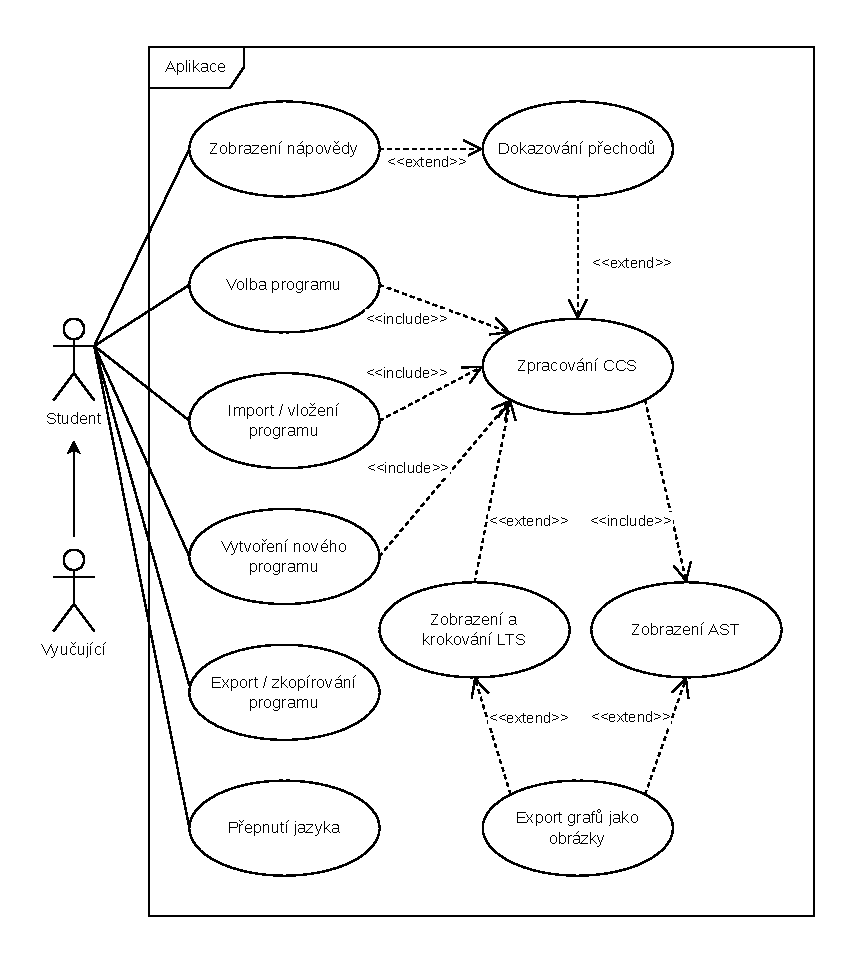
\includegraphics[width=0.93\textwidth]{Figures/usecase.pdf}
    \caption{UML diagram hlavních případů užití aplikace}
    \label{fig:use_case}
\end{figure}

\section{Návrh datových struktur}

Pro efektivní abstrakci jednotlivých komponent aplikace bylo nutné navrhnout datové toky a vnitřní reprezentaci uživatelských vstupů. 
Z uživatelského hlediska aplikace přijímá jako vstup textovou definici CCS procesů. 
Tento vstup je v první fázi zpracován syntaktickým analyzátorem, který vstupní text transformuje do abstraktního syntaktického stromu ve formátu JSON. 

Nad tímto stromem jsou posléze vystavěny další datové struktury nezbytné pro vnitřní logiku aplikace. 
Jedná se především o struktury pro generování vrcholů a hran grafu LTS, syntaktického stromu a struktury pro dokazování přechodů pomocí SOS pravidel. 
Detailní popis těchto struktur a procesu parsování je podrobněji rozebrán v kapitole \ref{sec:struct_format}.

\section{Architektura webové aplikace}

Aplikace je navržena jako Single-Page Application (SPA) s využitím knihovny React.js. 
Celý návrh dodržuje princip oddělení zodpovědností (Separation of Concerns). 
Zdrojové kódy a aplikační logika jsou logicky rozděleny do dvou hlavních vrstev, reprezentovaných adresářovou strukturou projektu:
\begin{itemize}
    \item \textbf{Vrstva aplikační logiky (adresář \texttt{lib}):} 
    Zajišťuje zapouzdření doménové logiky celého systému. 
    Obsahuje pouze funkce, které nejsou závislé na uživatelském rozhraní. 
    Nachází se zde například zpracování uživatelského vstupu, generátor syntaktického stromu či algoritmy pro výpočet stavových prostorů i přechodů pro LTS, včetně přípravy struktury pro následné vykreslení grafu.
    \item \textbf{Vrstva uživatelského rozhraní (adresář \texttt{components}):} 
    Vrstva sdružuje veškeré vizuální a interaktivní prvky aplikace, navržené jako znovupoužitelné komponenty.
    Součástí této vrstvy jsou také UI prvky z knihovny \texttt{shadcn/ui}, které tak mohou být funkčně přizpůsobeny potřebám projektu.
\end{itemize}

Základní adresář komponent je dále hierarchicky členěn podle své funkčnosti, viz obrázek \ref{fig:component_structure}. 
Mezi základní funkční celky patří \texttt{TextEditor}, obalující knihovnu CodeMirror pro zápis CCS a syntakticky strom, \texttt{SOSProofer} pro vše potřebné z oblasti interaktivní konstrukce důkazů a \texttt{LTSGraph} pro všechny komponenty specifické pro zobrazení LTS grafu. 
Klíčovou roli hraje \texttt{ProgramsContext}, který centralizovaně spravuje stavy aplikace jakožto jediný zdroj pravdy (Single Source of Truth). Tímto přístupem se zamezuje desynchronizaci dat napříč komponentami.
Veškeré úkony spojené s globální správou programů, jako je jejich vytváření, aktualizace, mazání a obecně práce s dynamicky generovanými kartami, jsou zpracovávany komponentami z \texttt{ProgramsSelector}.

\begin{figure}[h!]
    \centering
    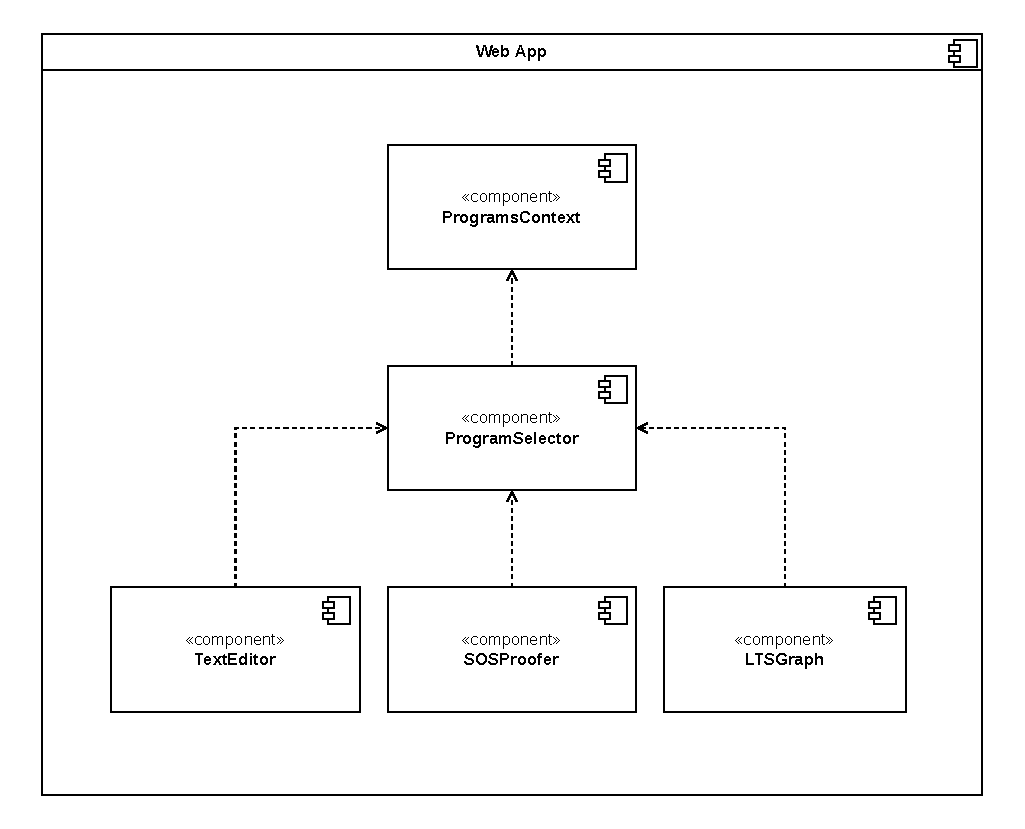
\includegraphics[width=0.95\textwidth]{Figures/components.pdf}
    \caption{UML diagram architektury aplikace}
    \label{fig:component_structure}
\end{figure}

\section{Uživatelské rozhraní}

Návrh uživatelského rozhraní klade důraz na interaktivitu, plynulost a přehlednost. 
Uživatelské prostředí se skládá z jediné dynamické stránky, jejíž obsah je spravován prostřednictvím překryvných modálních oken a variabilního systému karet, zobrazených na obrázku \ref{fig:card_ui}.

\begin{figure}[h!]
    \centering
    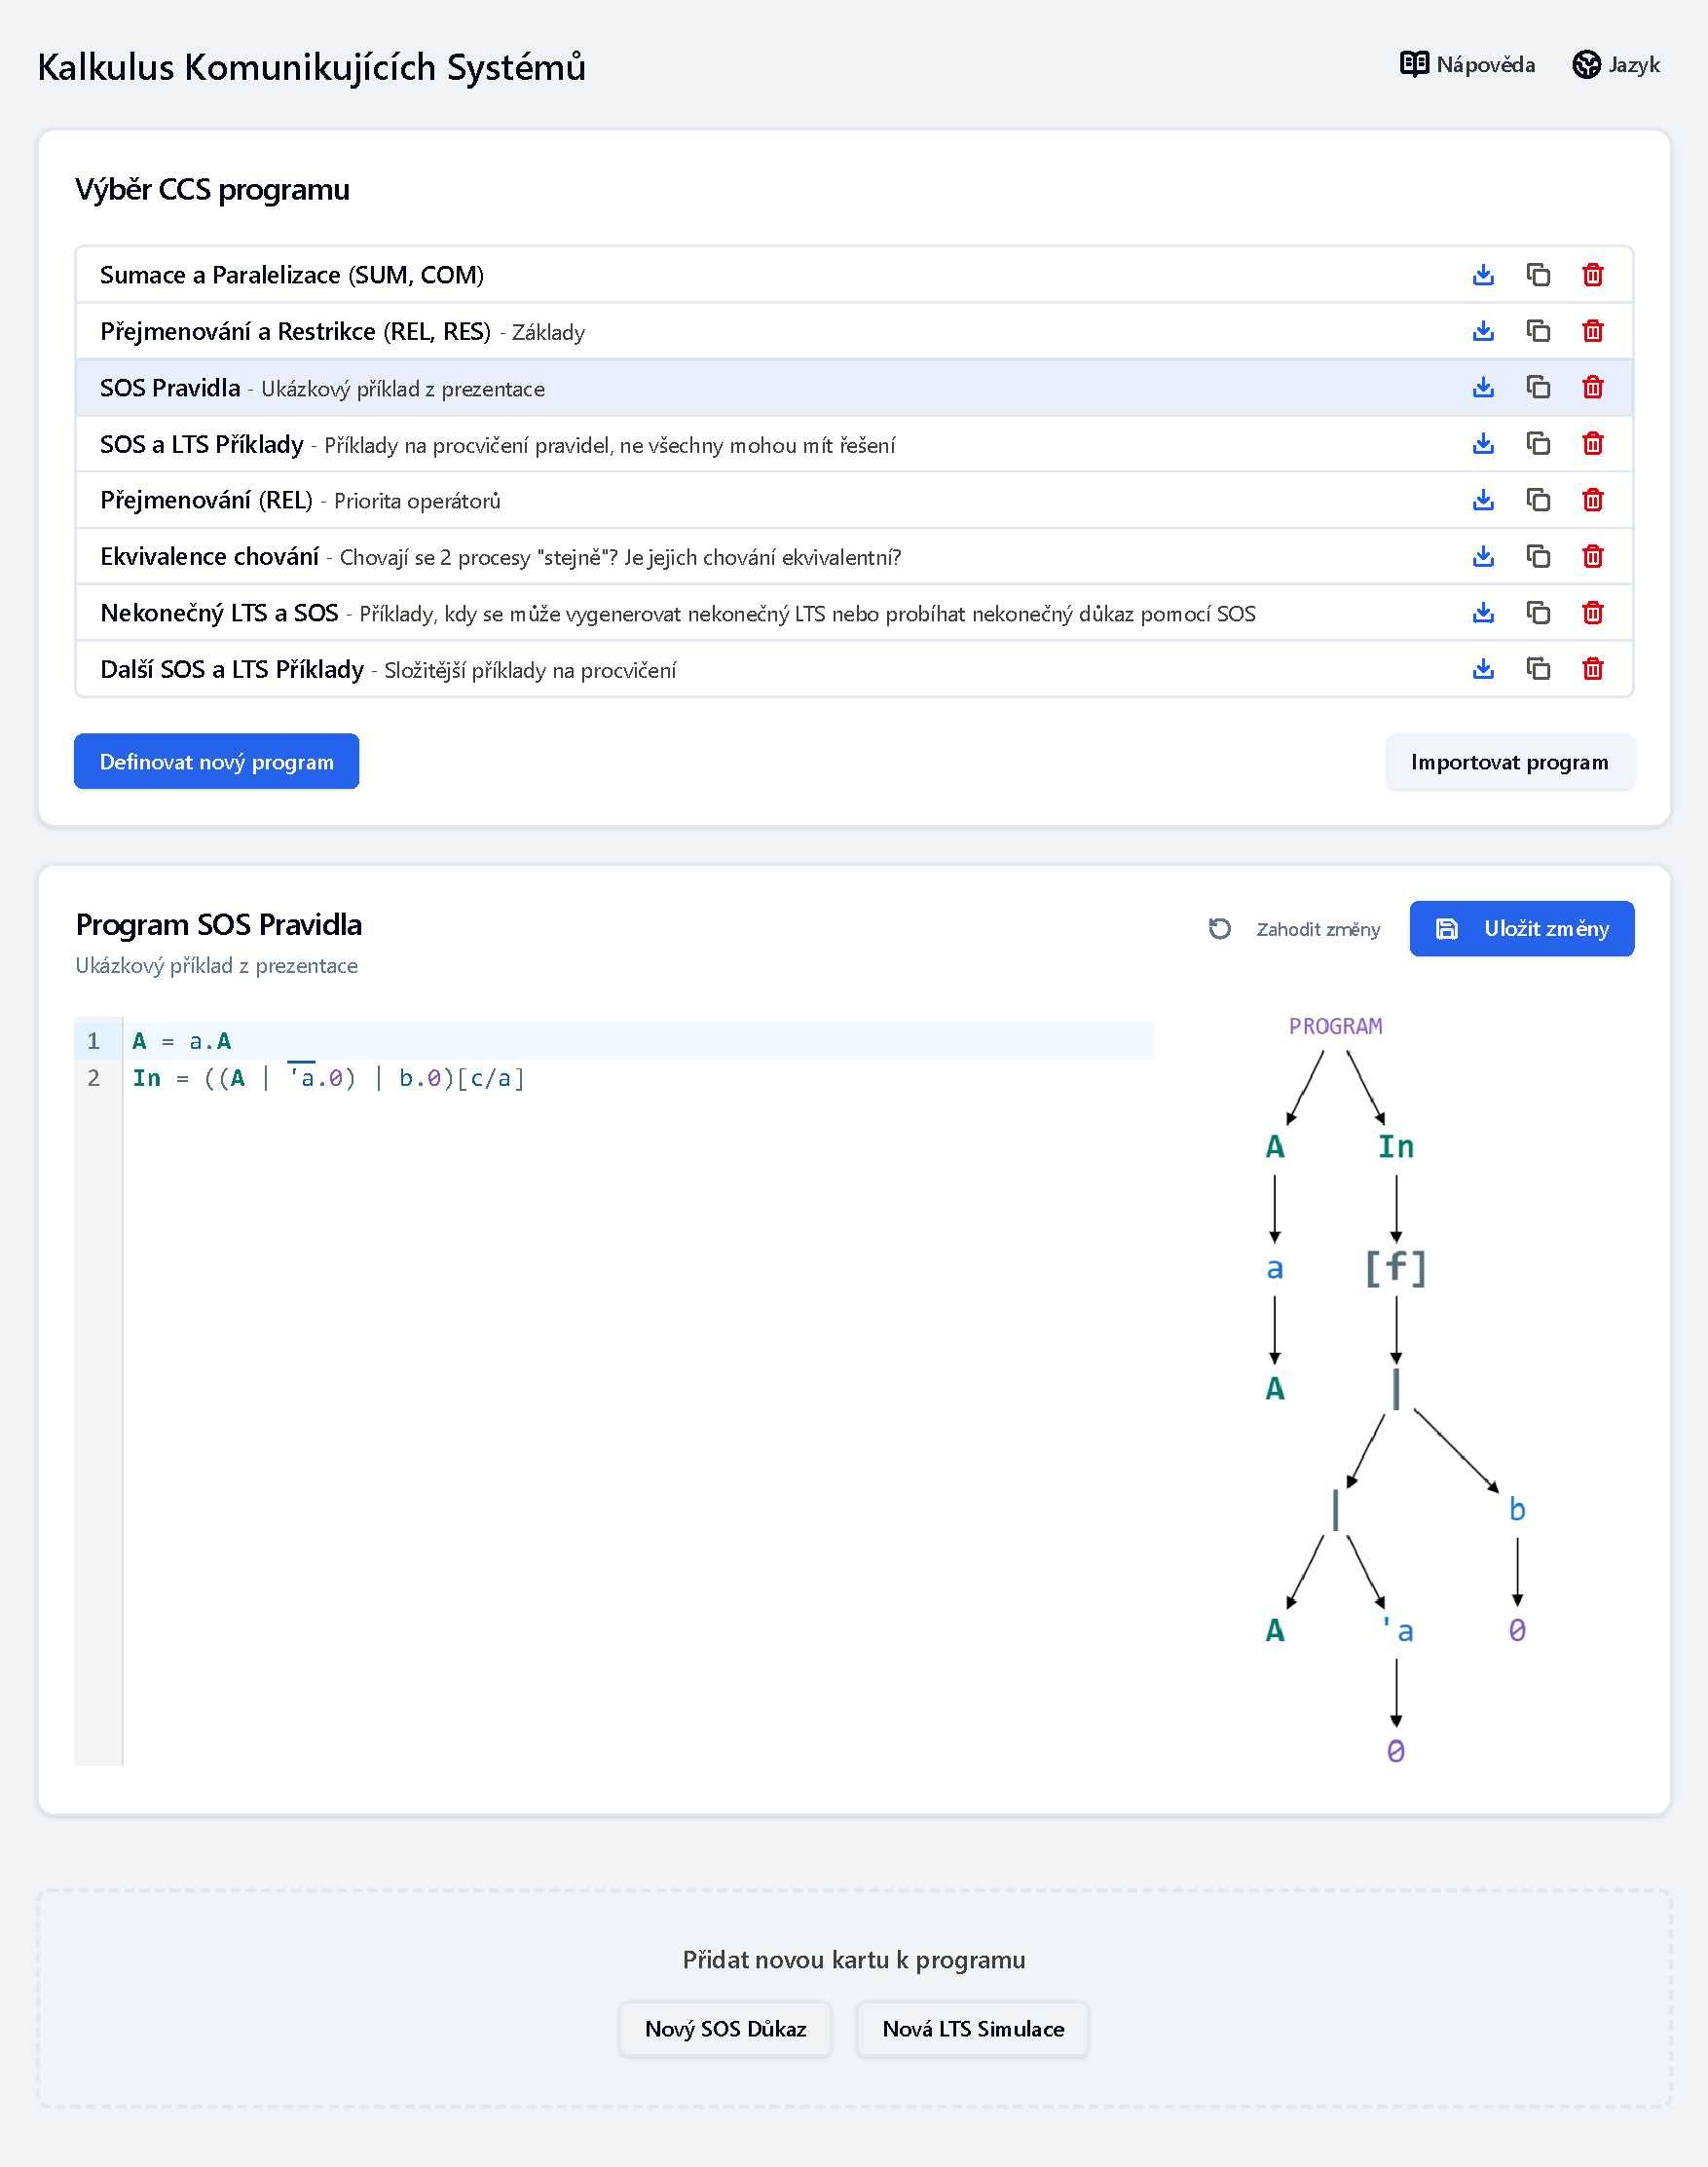
\includegraphics[width=0.98\textwidth]{Figures/card_ui.pdf}
    \caption{Uživatelské rozhraní založené na systému karet}
    \label{fig:card_ui}
\end{figure}

Při úvodním načtení aplikace vidí uživatel pouze výchozí kartu určenou k výběru programu. 
Zde má uživatel možnost načíst již vytvořený program, importovat vlastní zadání, nebo přes dialogové okno vytvořit program zcela nový. 
Hlavička stránky zůstává neměnná a nabízí změnu lokalizace i vyvolání nápovědy.

Jakmile je program zvolen či vytvořen, systém dynamicky vygeneruje hierarchicky podřazené karty. 
Výchozím a trvale přítomným prvkem je karta textového editoru. 
Uživatel v ní zadává definice procesů CCS, přičemž editor v reálném čase provádí validaci vstupu a graficky upozorňuje na případné syntaktické chyby. 
Při úspěšné validaci výrazu se ve stejné kartě rovněž automaticky vykresluje struktura syntaktického stromu.
Kromě textového editoru může k jednomu programu náležet libovolné množství dalších podkaret. Ty mohou být dvou typů:
\begin{enumerate}
    \item \textbf{Karta důkazu SOS:} 
    Nabízí interaktivní prostředí pro krokovou konstrukci důkazu přechodu z jednoho CCS výrazu do druhého za využití formálních pravidel strukturální operační sémantiky.
    \item \textbf{Karta LTS:} 
    Zajišťuje vizualizaci ohodnocených přechodových systémů, kde jednotlivé vrcholy grafu reprezentují dosažitelné stavy programu a hrany odpovídají akcím, které mění jeho stav.
\end{enumerate}

Na konci zobrazení podkaret je umístěna silueta karty, fungující jako rozcestník pro přidávání dalších karet obou zmíněných typů. 
Aby si uživatel udržel orientaci při vysokém počtu karet, umožňuje rozhraní každou z nich individuálně pojmenovat (funkcí editace v pravém horním rohu karty) a popsat tak, jakou konkrétní část systému daná karta vizualizuje či dokazuje. 
U vybraných karet je také dostupná nápověda pro specifické funkce karty. 
V případě, že je program explicitně uzamčen proti úpravám, přejde uživatelské rozhraní do režimu pouze pro čtení, kde není možné měnit obsah editoru a nelze jakkoli manipulovat s kartami.

\endinput

\chapter{Implementace}
\label{sec:implementace}

\section{Uživatelské rozhraní a logika aplikace}

\subsection{Výběr a správa programů}

\subsection{Karta textového editoru}

\subsection{Karta důkazu přechodů pomocí SOS pravidel}

\subsection{Karta zobrazení a krokování LTS grafu}
\label{sec:theory_dagre}

\section{Komunikace mezi komponentami}

\subsection{Programs store}

\subsection{Formát zpracovaného CCS výrazu}
\label{sec:struct_format}

\section{Možné úpravy aplikace}

\subsection{Přidání nových definic předdefinovaných programů}

\subsection{Lokalizace}

\section{Kompilace a nasazení}

\section{Optimalizace}

\subsection{Rychlost, Přístupnost, SEO}

\subsection{Vite komprimace}

\section{Možná vylepšení}

\endinput
\chapter{Závěr}

Cílem této diplomové práce bylo navrhnout a implementovat interaktivní aplikaci, která usnadní výuku a pochopení vybraných problémů z oblasti formální verifikace systémů. 
Konkrétní zaměření práce směřovalo na kalkulus komunikujících systémů, strukturální operační sémantiku a ohodnocené přechodové systémy. 
Tento cíl se podařilo v plném rozsahu naplnit vytvořením moderní a uživatelsky přívětivé webové aplikace.

V rámci teoretické a analytické části byly nejprve nastudovány principy reaktivních systémů a identifikovány nedostatky stávajících nástrojů v kontextu výuky začátků. 
Na základě těchto poznatků byla navržena aplikace, která uživatelům poskytuje okamžitou vizuální zpětnou vazbu a~provází je tak procesem formální modelace krok za krokem. 

Z technologického hlediska byla aplikace postavena na moderních tenchologiích, jako je React.js, TypeScript a Vite. 
Systém karet a modulární oddělení prezentační vrstvy od výpočetního jádra navíc zajišťují přehlednost, stabilitu a jednoduchou rozšiřitelnost celého řešení, což si myslím, že~je~velké plus této aplikace. 
Při vývoji aplikace jsem hlouběji pochopil problematiku komunikujících systémů, naučil jsem se ale také pracovat s několika moderními knihovnami, jako je Peggy.js a~Cytoscape.js. 
Jak již bylo nastíněno, užitečným rozšířením aplikace by mohla být implementace modulů pro ověřování silné a slabé ekvivalence chování (bisimulace) či integrace nástrojů pro model checking s~využitím Hennessy-Milnerovy logiky.


\endinput

% Seznam literatury
\printbibliography[title={Literatura}, heading=bibintoc]

% Prilohy
\appendix
\chapter{Popis adresářové struktury}
TODO, prozatím překopírováno z mé bakalářské práce.

% Návod na zprovoznění Latex na Windows

\dirtree{%
.1 /\DTcomment{Kořenový adresář}.
.2 esp32\DTcomment{Adresář základny}.
.3 main\DTcomment{Zdrojový kód základny}.
.2 mobile\_app\DTcomment{Adresář mobilní aplikace}.
.3 assets\DTcomment{Zdroje aplikace}.
.4 icons\DTcomment{Adresář ikon}.
.3 components\DTcomment{Komponenty}.
.4 addKey\DTcomment{Komponenty strany přídání klíče}.
.4 adminScreen\DTcomment{Komponenty admin stránky}.
.4 doorDetail\DTcomment{Komponenty detailu dveří}.
.4 layout\DTcomment{Základní komponenty}.
.3 constants\DTcomment{Konstanty, např. barvy, obrázky a stíny}.
.3 screens\DTcomment{Komponenty stránek aplikace}.
.3 types\DTcomment{Definice datových typů}.
.3 utilities\DTcomment{Vlastní hooks}.
}

\endinput

\end{document}
